\documentclass[tikz]{standalone}


%graphics

\usepackage{tikz}
\usetikzlibrary{shapes.geometric, shapes.multipart, arrows, calc, through,intersections}


\begin{document}


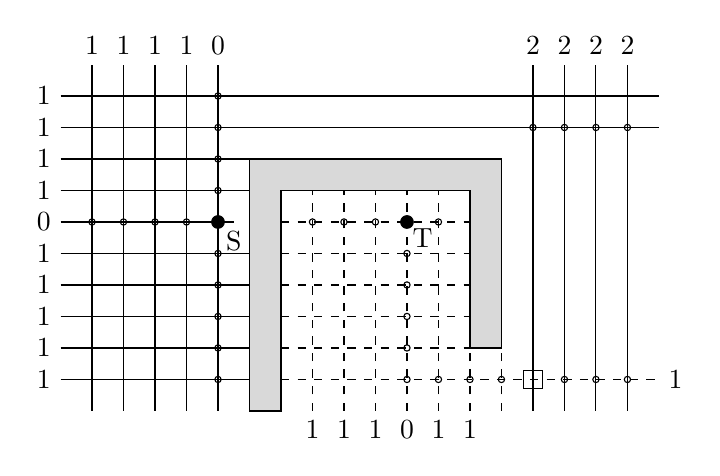
\begin{tikzpicture}[scale=0.4]

\draw (0,1) node[left]{1}-- (6,1);
\draw (0,2) node[left]{1}-- (6,2);
\draw (0,3) node[left]{1}-- (6,3);
\draw (0,4) node[left]{1}-- (6,4);
\draw (0,5) node[left]{1}-- (6,5);
\draw (0,6) node[left]{0}-- (5.5,6) node[below]{S};
\draw (0,7) node[left]{1}-- (6,7);
\draw (0,8) node[left]{1}-- (6,8);
\draw (0,9) node[left]{1}-- (19,9);
\draw (0,10)node[left]{1}-- (19,10);

\draw[fill=gray!30] (6,0) -- ++(1,0) -- ++(0,7) -- ++(6,0) -- ++(0,-5) -- ++(1,0) -- ++(0,6) -- ++(-8,0) -- cycle; 

\draw[dashed] (7,1) -- ++(12, 0)node[right]{1};
\draw[dashed] (7,2) -- ++(6,0);
\draw[dashed] (7,3) -- ++(6,0);
\draw[dashed] (7,4) -- ++(6,0);
\draw[dashed] (7,5) -- ++(6,0);
\draw[dashed] (7,6) -- ++(6,0);

\draw (1,0) -- ++(0,11) node[above]{1};
\draw (2,0) -- ++(0,11) node[above]{1};
\draw (3,0) -- ++(0,11) node[above]{1};
\draw (4,0) -- ++(0,11) node[above]{1};
\draw (5,0) -- ++(0,11) node[above]{0};

\draw (1,6) circle[radius=0.1cm];
\draw (2,6) circle[radius=0.1cm];
\draw (3,6) circle[radius=0.1cm];
\draw (4,6) circle[radius=0.1cm];
\draw[fill](5,6) circle[radius=0.2cm];
\draw(5,5) circle[radius=0.1cm];
\draw(5,4) circle[radius=0.1cm];
\draw(5,3) circle[radius=0.1cm];
\draw(5,2) circle[radius=0.1cm];
\draw(5,1) circle[radius=0.1cm];
\draw(5,7) circle[radius=0.1cm];
\draw(5,8) circle[radius=0.1cm];
\draw(5,9) circle[radius=0.1cm];
\draw(5,10) circle[radius=0.1cm];

\draw[dashed] (8,0)node[below]{1} -- ++(0,7);
\draw[dashed] (9,0)node[below]{1} -- ++(0,7);
\draw[dashed] (10,0)node[below]{1} -- ++(0,7);
\draw[dashed] (11,0)node[below]{0} -- ++(0,7);
\draw[dashed] (12,0)node[below]{1} -- ++(0,7);
\draw[dashed] (13,0)node[below]{1} -- ++(0,2);
\draw[dashed] (14,0) -- ++(0,2);

\draw(8,6) circle[radius=0.1cm];
\draw(9,6) circle[radius=0.1cm];
\draw(10,6) circle[radius=0.1cm];
\draw[fill](11,6) circle[radius=0.2cm];
\node at (11.5, 5.5) {T};
\draw(12,6) circle[radius=0.1cm];
\draw(11,5) circle[radius=0.1cm];
\draw(11,4) circle[radius=0.1cm];
\draw(11,3) circle[radius=0.1cm];
\draw(11,2) circle[radius=0.1cm];
\draw(11,1) circle[radius=0.1cm];
\draw(12,1) circle[radius=0.1cm];
\draw(13,1) circle[radius=0.1cm];
\draw(14,1) circle[radius=0.1cm];

\draw (15,0) -- ++ (0,11)node[above]{2};
\draw (16,0) -- ++ (0,11)node[above]{2};
\draw (17,0) -- ++ (0,11)node[above]{2};
\draw (18,0) -- ++ (0,11)node[above]{2};

\draw(15,9) circle[radius=0.1cm];
\draw(16,9) circle[radius=0.1cm];
\draw(17,9) circle[radius=0.1cm];
\draw(18,9) circle[radius=0.1cm];
\draw(15,1) node [draw, rectangle]{};
\draw(16,1) circle[radius=0.1cm];
\draw(17,1) circle[radius=0.1cm];
\draw(18,1) circle[radius=0.1cm];
\end{tikzpicture}
\end{document}
